\documentclass[11pt,a4paper]{article}
\usepackage[utf8]{inputenc}
\usepackage[T1]{fontenc}
\usepackage{lmodern}
\usepackage[french]{babel}
\usepackage[margin=2.3cm]{geometry}
\usepackage{amsmath,amssymb,mathtools}
\usepackage{bm}
\usepackage{graphicx}
\usepackage{booktabs}
\usepackage{enumitem}
\usepackage[dvipsnames]{xcolor}
\usepackage[most]{tcolorbox}
\usepackage{listings}
\usepackage{hyperref}
\hypersetup{colorlinks=true,linkcolor=NavyBlue,urlcolor=NavyBlue}
\usepackage{fancyhdr}
\pagestyle{fancy}\fancyhf{}
\lhead{\small ECN-7025 -- Devoir 1 (automne 2026)}\rhead{\small Solutions détaillées}\cfoot{\thepage}
\setlength{\headheight}{14pt}
\setlength{\parskip}{0.45em}\setlength{\parindent}{0pt}

\newcommand{\vy}{\mathbf{y}}\newcommand{\vX}{\mathbf{X}}\newcommand{\vZ}{\mathbf{Z}}
\newcommand{\ve}{\mathbf{e}}\newcommand{\vb}{\mathbf{b}}\newcommand{\vc}{\mathbf{c}}
\newcommand{\vbeta}{\bm{\beta}}\newcommand{\veps}{\bm{\epsilon}}\newcommand{\valpha}{\bm{\alpha}}
\newcommand{\A}{\mathbf{A}}\newcommand{\I}{\mathbf{I}}
\newcommand{\Pm}{\mathbf{P}}\newcommand{\vx}{\mathbf{x}}\newcommand{\Mz}{\mathbf{M}_Z}\newcommand{\Pz}{\mathbf{P}_Z}
\newcommand{\tX}{\tilde{\mathbf{X}}}
\newcommand{\E}{\mathbb{E}}\newcommand{\Var}{\operatorname{Var}}\newcommand{\Cov}{\operatorname{Cov}}
\newcommand{\sumi}{\sum_{i=1}^{n}}

\newtcolorbox{idee}[1][]{colback=Cerulean!6,colframe=Cerulean!70!black,fonttitle=\bfseries,title={Idée de la démarche},#1}
\newtcolorbox{reponse}[1][]{colback=ForestGreen!6,colframe=ForestGreen!70!black,fonttitle=\bfseries,title={Réponse},#1}
\newtcolorbox{attention}[1][]{colback=BrickRed!5,colframe=BrickRed!75!black,fonttitle=\bfseries,title={Attention},#1}
\newtcolorbox{intuition}[1][]{colback=Goldenrod!8,colframe=Goldenrod!70!black,fonttitle=\bfseries,title={Intuition},#1}

\lstset{basicstyle=\ttfamily\small,breaklines=true,frame=single,backgroundcolor=\color{gray!6},
  columns=fullflexible,keepspaces=true,showstringspaces=false,
  literate={é}{{\'e}}1 {è}{{\`e}}1 {à}{{\`a}}1 {ê}{{\^e}}1 {ç}{{\c{c}}}1 {É}{{\'E}}1 {ù}{{\`u}}1 {ô}{{\^o}}1 {î}{{\^i}}1}

\begin{document}

\begin{center}
{\LARGE\bfseries ECN-7025 Économétrie I -- Devoir 1}\\[4pt]
{\large Solutions détaillées, démarche pas à pas et explications}\\[4pt]
{\small Chapitre 2 (MCO) -- Greene, ch. 3 et 4}
\end{center}

\begin{tcolorbox}[colback=white,colframe=NavyBlue,title=Comment lire ce document]
Pour chaque question : \textbf{l'idée de la démarche} (quoi faire et pourquoi), puis la \textbf{démonstration ou le calcul complet}, puis la \textbf{réponse} encadrée et, quand c'est utile, une \textbf{intuition}.
Les numéros « [$n$] » renvoient aux équations des notes du chapitre 2.

\textbf{Codes fournis} : \texttt{stata/devoir1.do} (questions 3 et 4). Les résultats numériques présentés ici ont été calculés en Python (voir la note en début des questions 3 et 4) ; à reproduire avec le do-file sur vos propres fichiers avant de remettre le devoir.
\end{tcolorbox}

\tableofcontents

% =====================================================================
\section{Question 1 (25 points)}
% =====================================================================

\subsection{(a)(i) Changement de base des régresseurs : $\tilde{\vb}=\A^{-1}\vb$}

\begin{idee}
On écrit la formule des MCO pour le modèle transformé, $\tilde{\vb}=(\tX'\tX)^{-1}\tX'\vy$, on remplace $\tX$ par $\vX\A$, puis on utilise deux règles d'algèbre : $(\vX\A)'=\A'\vX'$ et l'inverse d'un produit de matrices carrées inversibles, $(\mathbf{BCD})^{-1}=\mathbf{D}^{-1}\mathbf{C}^{-1}\mathbf{B}^{-1}$.
\end{idee}

\textbf{Hypothèses utilisées.} $\vX$ ($n\times k$) est de plein rang colonne, donc $\vX'\vX$ ($k\times k$) est inversible et $\vb=(\vX'\vX)^{-1}\vX'\vy$ existe. $\A$ ($k\times k$) est non singulière, donc $\A^{-1}$ et $(\A')^{-1}=(\A^{-1})'$ existent.

\textbf{Étape 1 : $\tX$ est aussi de plein rang}, donc $\tilde{\vb}$ existe. Si $\tX\mathbf{v}=\vX(\A\mathbf{v})=\mathbf 0$, le plein rang de $\vX$ donne $\A\mathbf{v}=\mathbf 0$, et comme $\A$ est inversible, $\mathbf{v}=\mathbf 0$.

\textbf{Étape 2 : calcul.}
\begin{align*}
\tilde{\vb}&=(\tX'\tX)^{-1}\tX'\vy\\
&=\big((\vX\A)'(\vX\A)\big)^{-1}(\vX\A)'\vy
 &&\text{définition de }\tX\\
&=\big(\A'\,(\vX'\vX)\,\A\big)^{-1}\A'\vX'\vy
 &&(\vX\A)'=\A'\vX'\\
&=\A^{-1}(\vX'\vX)^{-1}(\A')^{-1}\,\A'\vX'\vy
 &&\text{inverse d'un produit de 3 matrices } k\times k \text{ inversibles}\\
&=\A^{-1}(\vX'\vX)^{-1}\underbrace{(\A')^{-1}\A'}_{=\I_k}\vX'\vy\\
&=\A^{-1}\underbrace{(\vX'\vX)^{-1}\vX'\vy}_{=\vb}=\A^{-1}\vb .
\end{align*}

\begin{reponse}
$\tilde{\vb}=\A^{-1}\vb$. \hfill$\blacksquare$
\end{reponse}

\textbf{Conséquences utiles (à mentionner pour la partie (ii)).}
\begin{itemize}[nosep]
\item \emph{Valeurs prédites et résidus inchangés} : $\tX\tilde{\vb}=\vX\A\A^{-1}\vb=\vX\vb=\hat{\vy}$, donc $\tilde{\ve}=\ve$, même SCE, même $s^2$, même $R^2$.
\item \emph{Variance} : $\widehat{\Var}(\tilde{\vb})=s^2(\tX'\tX)^{-1}=s^2\A^{-1}(\vX'\vX)^{-1}(\A^{-1})'=\A^{-1}\,\widehat{\Var}(\vb)\,(\A^{-1})'$.
\end{itemize}

\begin{intuition}
$\tX=\vX\A$ a exactement les mêmes colonnes « en combinaisons linéaires » que $\vX$ : l'espace engendré par les colonnes est le même. Or les MCO projettent $\vy$ sur cet espace ($\hat{\vy}=\Pm\vy$) ; la projection ne change donc pas, seule la façon d'écrire $\hat{\vy}$ comme combinaison des colonnes change. Les coefficients s'ajustent pour compenser : c'est $\A^{-1}$.
\end{intuition}

\subsection{(a)(ii) Salaire mesuré en cents au lieu de dollars}

\begin{idee}
Passer de dollars à cents revient à multiplier la colonne $x$ par 100 sans toucher à la constante. C'est un cas particulier de $\tX=\vX\A$ avec une matrice $\A$ diagonale. On applique (i).
\end{idee}

Ici $\vX=[\bm\iota\ \ \mathbf x]$ ($n\times 2$) et la nouvelle variable est $x_i^{c}=100\,x_i$. Donc
\[
\tX=[\bm\iota\ \ 100\mathbf x]=[\bm\iota\ \ \mathbf x]\underbrace{\begin{pmatrix}1&0\\0&100\end{pmatrix}}_{\A},
\qquad
\A^{-1}=\begin{pmatrix}1&0\\0&1/100\end{pmatrix}.
\]
Par (i) :
\[
\begin{pmatrix}\tilde b_0\\ \tilde b_1\end{pmatrix}=\A^{-1}\begin{pmatrix}b_0\\ b_1\end{pmatrix}=\begin{pmatrix}b_0\\ b_1/100\end{pmatrix}.
\]

\begin{reponse}
\begin{itemize}[nosep]
\item \textbf{Pente} : $\tilde b_1=b_1/100$. Si $b_1$ = variation des heures hebdomadaires pour une hausse du salaire horaire de 1 \$, alors $\tilde b_1$ = variation pour une hausse de 1 cent, qui est 100 fois plus petite. Exemple : $b_1=0{,}5$ heure par dollar devient $\tilde b_1=0{,}005$ heure par cent. \textbf{L'effet économique est identique} ; seule l'unité change.
\item \textbf{Constante} : inchangée ($\tilde b_0=b_0$), car la colonne de 1 n'est pas modifiée ; un salaire nul vaut 0 en dollars comme en cents.
\item \textbf{Écart-type} : $\widehat{\Var}(\tilde{\vb})=\A^{-1}\widehat{\Var}(\vb)\A^{-1}$ donne $\text{e.t.}(\tilde b_1)=\text{e.t.}(b_1)/100$. Donc \textbf{la statistique $t$} ($\tilde b_1/\text{e.t.}(\tilde b_1)=b_1/\text{e.t.}(b_1)$), la $p$-value, les résidus et le $R^2$ sont \textbf{inchangés}.
\end{itemize}
Moralité : les unités de mesure n'affectent ni l'ajustement ni l'inférence ; elles changent seulement l'échelle (la lecture) des coefficients.
\end{reponse}

\begin{attention}
Si l'on changeait plutôt l'unité de $y$ (heures $\to$ minutes, facteur 60), \emph{tous} les coefficients seraient multipliés par 60. Et si $x$ entrait en logarithme, $\ln(100x)=\ln 100+\ln x$ : la pente ne changerait pas mais la constante oui. On le reverra à la question 4 : \texttt{lwage} est en log, donc l'unité du salaire (dollars ou cents) n'affecte que la constante.
\end{attention}

% ---------------------------------------------------------------------
\subsection{(b) Même somme des carrés des résidus pour (3) et (4)}

Modèles : \quad (3) $\vy=\vX\vbeta+\vZ\bm\gamma+\veps$, \qquad (4) $\Mz\vy=\Mz\vX\vbeta+\tilde{\veps}$, \quad avec $\Mz=\I_n-\vZ(\vZ'\vZ)^{-1}\vZ'$.

\begin{idee}
On montre plus fort que demandé : \textbf{les vecteurs de résidus sont identiques}. L'égalité de la somme (et de la somme des carrés) des résidus en découle immédiatement. Trois ingrédients :
\begin{enumerate}[nosep]
\item les équations normales de (3) ;
\item le théorème de Frisch-Waugh-Lovell (FWL), qu'on redémontre : le $\vb$ de (3) est égal au $\vb$ de (4) ;
\item les résidus de (3) sont orthogonaux à $\vZ$, donc $\Mz$ ne les modifie pas.
\end{enumerate}
\end{idee}

\textbf{Notation et hypothèse.} On suppose $\mathbf W=[\vX\ \vZ]$ de plein rang colonne. Soient $(\vb,\vc)$ les estimateurs MCO de (3) et $\ve=\vy-\vX\vb-\vZ\vc$ ses résidus. Soient $\tilde{\vb}$ l'estimateur MCO de (4) et $\tilde{\ve}=\Mz\vy-\Mz\vX\tilde{\vb}$ ses résidus.

\textbf{Rappel : propriétés de $\Mz$.} Symétrique ($\Mz'=\Mz$), idempotente ($\Mz\Mz=\Mz$), et $\Mz\vZ=\mathbf 0$ (démontré dans les notes, §2.2).

\medskip
\textbf{Étape 1 : l'estimateur MCO de (4).} Par la formule générale appliquée aux données transformées,
\[
\tilde{\vb}=\big((\Mz\vX)'(\Mz\vX)\big)^{-1}(\Mz\vX)'(\Mz\vy)=(\vX'\Mz'\Mz\vX)^{-1}\vX'\Mz'\Mz\vy=(\vX'\Mz\vX)^{-1}\vX'\Mz\vy .
\]
Il existe car $\vX'\Mz\vX$ est inversible. En effet, si $\Mz\vX\mathbf v=\mathbf 0$, alors $\vX\mathbf v=\Pz\vX\mathbf v=\vZ\mathbf d$ avec $\mathbf d=(\vZ'\vZ)^{-1}\vZ'\vX\mathbf v$. Donc $\vX\mathbf v-\vZ\mathbf d=\mathbf 0$, et le plein rang de $\mathbf W$ impose $\mathbf v=\mathbf 0$.

\textbf{Étape 2 : les équations normales de (3).} Elles s'écrivent $\mathbf W'\ve=\mathbf 0$, c'est-à-dire
\begin{align}
\vX'\ve&=\mathbf 0 \iff \vX'\vX\vb+\vX'\vZ\vc=\vX'\vy, \tag{N1}\\
\vZ'\ve&=\mathbf 0 \iff \vZ'\vX\vb+\vZ'\vZ\vc=\vZ'\vy. \tag{N2}
\end{align}

\textbf{Étape 3 : FWL, $\vb=\tilde{\vb}$.} De (N2) : $\vc=(\vZ'\vZ)^{-1}\vZ'(\vy-\vX\vb)$. On substitue dans (N1) :
\[
\vX'\vX\vb+\vX'\underbrace{\vZ(\vZ'\vZ)^{-1}\vZ'}_{\Pz}(\vy-\vX\vb)=\vX'\vy
\]
\[
\iff \vX'(\I-\Pz)\vX\,\vb=\vX'(\I-\Pz)\vy
\iff \vX'\Mz\vX\,\vb=\vX'\Mz\vy .
\]
Donc $\vb=(\vX'\Mz\vX)^{-1}\vX'\Mz\vy=\tilde{\vb}$.

\textbf{Étape 4 : $\Mz\ve=\ve$.} Par (N2), $\vZ'\ve=\mathbf 0$, donc $\Pz\ve=\vZ(\vZ'\vZ)^{-1}\vZ'\ve=\mathbf 0$ et $\Mz\ve=\ve-\Pz\ve=\ve$.

\textbf{Étape 5 : conclusion.} On prémultiplie la décomposition $\vy=\vX\vb+\vZ\vc+\ve$ par $\Mz$ :
\[
\Mz\vy=\Mz\vX\vb+\underbrace{\Mz\vZ}_{\mathbf 0}\vc+\underbrace{\Mz\ve}_{\ve}
\quad\Longrightarrow\quad
\ve=\Mz\vy-\Mz\vX\vb=\Mz\vy-\Mz\vX\tilde{\vb}=\tilde{\ve}\quad(\text{étape 3}).
\]

\begin{reponse}
Les résidus des deux régressions sont \textbf{le même vecteur} : $\ve=\tilde{\ve}$. Par conséquent
\[
\ve'\ve=\tilde{\ve}'\tilde{\ve}\qquad\text{et aussi}\qquad \textstyle\sum_i e_i=\sum_i\tilde e_i .
\]
Les sommes des carrés des résidus MCO de (3) et de (4) sont égales. \hfill$\blacksquare$
\end{reponse}

\begin{intuition}
$\Mz$ « nettoie » $\vy$ et $\vX$ de tout ce que $\vZ$ explique. Une fois $\vZ$ retiré des deux côtés, il ne reste plus rien que $\vZ$ puisse expliquer : l'inclure explicitement (modèle 3) ou l'avoir retiré au préalable (modèle 4) laisse exactement la même partie inexpliquée de $\vy$.
\end{intuition}

\begin{attention}
Les SCE sont égales, mais pas les \emph{degrés de liberté}. Le logiciel divise la SCE par $n-k$ pour (4) alors qu'il faut diviser par $n-k-m$ (où $m$ est le nombre de colonnes de $\vZ$), comme pour (3). Les écarts-types affichés pour la régression (4) sont donc un peu trop petits ; il faut les multiplier par $\sqrt{(n-k)/(n-k-m)}$.
\end{attention}

% ---------------------------------------------------------------------
\subsection{(c) Erreur de moyenne conditionnelle non nulle}

Modèle $y_i=\beta_0+\beta_1x_i+\epsilon_i$ avec $\E[\epsilon_i\mid x_i]=\alpha_0+\alpha_1x_i$.

\begin{idee}
Deux méthodes équivalentes : (1) réécrire le modèle avec une nouvelle erreur de moyenne conditionnelle nulle ; (2) calculer directement $\E[\vb\mid\vX]$ avec la décomposition $\vb=\vbeta+(\vX'\vX)^{-1}\vX'\veps$ du cours [79].
\end{idee}

\textbf{Méthode 1 : réécriture.} Posons $u_i=\epsilon_i-\E[\epsilon_i\mid x_i]=\epsilon_i-\alpha_0-\alpha_1x_i$. Par construction, $\E[u_i\mid x_i]=0$. Alors
\[
y_i=\beta_0+\beta_1x_i+\alpha_0+\alpha_1x_i+u_i=\underbrace{(\beta_0+\alpha_0)}_{\gamma_0}+\underbrace{(\beta_1+\alpha_1)}_{\gamma_1}x_i+u_i .
\]
Ce modèle satisfait l'hypothèse d'exogénéité, donc les MCO estiment sans biais $\gamma_0$ et $\gamma_1$.

\textbf{Méthode 2 : calcul direct} (avec un échantillon aléatoire, $\E[\epsilon_i\mid x_1,\dots,x_n]=\E[\epsilon_i\mid x_i]$). Le vecteur $\E[\veps\mid\vX]$ a pour $i$-ème composante $\alpha_0+\alpha_1x_i=\vx_i'\valpha$, avec $\valpha=(\alpha_0,\alpha_1)'$ : donc $\E[\veps\mid\vX]=\vX\valpha$. Alors
\[
\E[\vb\mid\vX]=\vbeta+(\vX'\vX)^{-1}\vX'\E[\veps\mid\vX]=\vbeta+(\vX'\vX)^{-1}\vX'\vX\valpha=\vbeta+\valpha .
\]

\begin{reponse}
\[
\gamma_0=\beta_0+\alpha_0,\qquad \gamma_1=\beta_1+\alpha_1 .
\]
Les MCO sont biaisés pour $\beta_0$ (biais $\alpha_0$) et pour $\beta_1$ (biais $\alpha_1$), mais sans biais pour $\gamma_0$ et $\gamma_1$.
\end{reponse}

\begin{intuition}
\begin{itemize}[nosep]
\item \textbf{$\alpha_0$ est inoffensif} : une erreur de moyenne constante non nulle est simplement absorbée par la constante. C'est pourquoi l'hypothèse $\E[\epsilon]=0$ n'est qu'une \emph{normalisation} quand le modèle contient une constante (voir question 4(b)).
\item \textbf{$\alpha_1$ est le vrai problème} : si l'erreur varie systématiquement avec $x$, les MCO attribuent à $x$ l'effet de ce qui est caché dans l'erreur. Exemple : dans une équation de salaire, si l'habileté (dans $\epsilon$) augmente avec l'éducation, alors $\alpha_1>0$ et les MCO surestiment le rendement de l'éducation. C'est le biais de variable omise (exercice 7 du document d'explications du chapitre 2).
\end{itemize}
\end{intuition}

% =====================================================================
\section{Question 2 (25 points)}
% =====================================================================

Modèle \textbf{sans constante} : $y_i=\beta x_i+\epsilon_i$, avec $\E[\epsilon_i\mid x_i]=0$, $\E[\epsilon_i\epsilon_j\mid x_i]=0$ ($i\ne j$) et $\Var(\epsilon_i\mid x_i)=\sigma^2$.
\[
b_{MCO}=\frac{\sumi x_iy_i}{\sumi x_i^2},\qquad
b_{MOM}=\frac{\widehat{\Cov}(Y,X)}{\widehat{\Var}(X)}=\frac{\sumi(x_i-\bar x)(y_i-\bar y)}{\sumi(x_i-\bar x)^2}.
\]
(Les facteurs $1/n$ ou $1/(n-1)$ de la covariance et de la variance empiriques s'annulent dans le rapport.)

\textbf{Conventions.} Comme dans le cours, on raisonne conditionnellement à toutes les $x$ (notées $\vX$), avec un échantillon aléatoire, de sorte que $\E[\epsilon_i\mid\vX]=0$, $\Var(\epsilon_i\mid\vX)=\sigma^2$ et $\Cov(\epsilon_i,\epsilon_j\mid\vX)=0$. On suppose que $x$ varie dans l'échantillon : $\sum(x_i-\bar x)^2>0$.

\textbf{Deux identités utiles} (car $\sum(x_i-\bar x)=0$) :
\[
\text{(I1)}\ \ \sumi(x_i-\bar x)(y_i-\bar y)=\sumi(x_i-\bar x)y_i,
\qquad
\text{(I2)}\ \ \sumi(x_i-\bar x)x_i=\sumi(x_i-\bar x)^2 .
\]
Preuve de (I1) : $\sum(x_i-\bar x)(y_i-\bar y)=\sum(x_i-\bar x)y_i-\bar y\sum(x_i-\bar x)=\sum(x_i-\bar x)y_i$. (I2) : même argument avec $x$ à la place de $y$.

\subsection{(a) Les deux estimateurs sont sans biais}

\begin{idee}
Comme en [79] : on remplace $y_i$ par $\beta x_i+\epsilon_i$ pour écrire chaque estimateur sous la forme « $\beta$ + combinaison linéaire des erreurs », puis on prend l'espérance conditionnelle.
\end{idee}

\textbf{$b_{MCO}$.}
\[
b_{MCO}=\frac{\sum x_i(\beta x_i+\epsilon_i)}{\sum x_i^2}=\beta\frac{\sum x_i^2}{\sum x_i^2}+\frac{\sum x_i\epsilon_i}{\sum x_i^2}=\beta+\sumi w_i\epsilon_i,\qquad w_i=\frac{x_i}{\sum_j x_j^2}.
\]
Les poids $w_i$ ne dépendent que des $x$, donc
$\E[b_{MCO}\mid\vX]=\beta+\sum w_i\,\E[\epsilon_i\mid\vX]=\beta+0=\beta$.

\textbf{$b_{MOM}$.} Par (I1), puis (I2) :
\[
b_{MOM}=\frac{\sum(x_i-\bar x)y_i}{\sum(x_i-\bar x)^2}
=\frac{\beta\sum(x_i-\bar x)x_i+\sum(x_i-\bar x)\epsilon_i}{\sum(x_i-\bar x)^2}
=\beta+\sumi k_i\epsilon_i,\qquad k_i=\frac{x_i-\bar x}{\sum_j(x_j-\bar x)^2}.
\]
D'où $\E[b_{MOM}\mid\vX]=\beta+\sum k_i\,\E[\epsilon_i\mid\vX]=\beta$.

\begin{reponse}
$\E[b_{MCO}\mid\vX]=\E[b_{MOM}\mid\vX]=\beta$. Par la loi des espérances itérées, $\E[b_{MCO}]=\E[b_{MOM}]=\beta$ : les deux estimateurs sont sans biais.
\end{reponse}

\begin{attention}
Le point subtil de $b_{MOM}$ est le terme en $\bar y$ : il disparaît grâce à (I1). Sans cette identité, on pourrait croire que $\bar y$ (qui contient $\bar\epsilon$) pose problème. Autre remarque : $b_{MOM}$ est sans biais ici \emph{même si} le vrai modèle avait une constante, ce qui n'est pas le cas de $b_{MCO}$ (voir (c)).
\end{attention}

\subsection{(b) $b_{MCO}$ est efficace par rapport à $b_{MOM}$}

\begin{idee}
« Efficace relativement » signifie : tous deux sont sans biais et $\Var(b_{MCO}\mid\vX)\le\Var(b_{MOM}\mid\vX)$. On calcule les deux variances à partir des écritures « $\beta+\sum(\text{poids})\epsilon_i$ », puis on les compare grâce à la décomposition $\sum x_i^2=\sum(x_i-\bar x)^2+n\bar x^2$.
\end{idee}

\textbf{Variance d'une combinaison linéaire des erreurs.} Pour des poids $a_i$ fonctions des $x$ :
\[
\Var\Big(\sum a_i\epsilon_i\,\Big|\,\vX\Big)=\sum_i a_i^2\underbrace{\Var(\epsilon_i\mid\vX)}_{\sigma^2}+\sum_{i\ne j}a_ia_j\underbrace{\Cov(\epsilon_i,\epsilon_j\mid\vX)}_{0}=\sigma^2\sum_i a_i^2 .
\]
(On utilise l'homoscédasticité et l'absence de corrélation entre les erreurs.)

\textbf{Application.}
\[
\Var(b_{MCO}\mid\vX)=\sigma^2\sum_i\frac{x_i^2}{(\sum_j x_j^2)^2}=\frac{\sigma^2}{\sumi x_i^2},
\]
\[
\Var(b_{MOM}\mid\vX)=\sigma^2\sum_i\frac{(x_i-\bar x)^2}{(\sum_j(x_j-\bar x)^2)^2}=\frac{\sigma^2}{\sumi(x_i-\bar x)^2}.
\]

\textbf{Comparaison.} Développons :
\[
\sumi x_i^2=\sumi\big((x_i-\bar x)+\bar x\big)^2=\sumi(x_i-\bar x)^2+2\bar x\underbrace{\sumi(x_i-\bar x)}_{0}+n\bar x^2=\sumi(x_i-\bar x)^2+n\bar x^2 .
\]
Donc $\sum x_i^2\ge\sum(x_i-\bar x)^2$, et en passant à l'inverse :
\[
\Var(b_{MCO}\mid\vX)=\frac{\sigma^2}{\sum(x_i-\bar x)^2+n\bar x^2}\ \le\ \frac{\sigma^2}{\sum(x_i-\bar x)^2}=\Var(b_{MOM}\mid\vX),
\]
avec inégalité \textbf{stricte} dès que $\bar x\ne0$.

\begin{reponse}
Les deux estimateurs sont sans biais et $\Var(b_{MCO}\mid\vX)\le\Var(b_{MOM}\mid\vX)$ : $b_{MCO}$ est efficace par rapport à $b_{MOM}$. Le rapport des variances vaut
\[
\frac{\Var(b_{MOM}\mid\vX)}{\Var(b_{MCO}\mid\vX)}=\frac{\sum x_i^2}{\sum(x_i-\bar x)^2}=1+\frac{\bar x^2}{\hat\sigma_x^2},\qquad \hat\sigma_x^2=\tfrac1n\textstyle\sum(x_i-\bar x)^2 .
\]
Exemple : si $\bar x=2$ et $\hat\sigma_x=1$, la variance de $b_{MOM}$ est \textbf{5 fois} plus grande. Il faudrait 5 fois plus d'observations pour atteindre la même précision.
\end{reponse}

\textbf{Autre démonstration (via Gauss-Markov).} $b_{MOM}=\sum k_iy_i$ est \emph{linéaire} en $y$, et on a montré en (a) qu'il est sans biais. Les hypothèses de Gauss-Markov sont vérifiées (le modèle est $\vy=\vX\beta+\veps$ avec $\vX=\mathbf x$, sans constante), et $b_{MCO}=(\mathbf x'\mathbf x)^{-1}\mathbf x'\vy$ est l'estimateur MCO de ce modèle. Le théorème garantit donc $\Var(b_{MCO}\mid\vX)\le\Var(b_{MOM}\mid\vX)$. En reprenant la notation du cours, $D=k-w$ et $\Var(b_{MOM})=\Var(b_{MCO})+\sigma^2\sum(k_i-w_i)^2$.

\subsection{(c) Intuition}

\begin{intuition}
\begin{itemize}
\item \textbf{$b_{MOM}$ n'utilise pas une information que l'on possède.} $b_{MOM}$ est exactement la pente MCO d'une régression de $y$ sur une constante \emph{et} $x$ (formule [16]). Il estime donc une constante alors que le modèle dit qu'elle vaut zéro : la droite doit passer par l'origine. Estimer un paramètre inutile coûte de la précision (même phénomène que la variable non pertinente de la question 3(b)).
\item \textbf{Il n'utilise qu'une partie de la variation de $x$.} $b_{MOM}$ n'exploite que la variation de $x$ \emph{autour de sa moyenne}, $\sum(x_i-\bar x)^2$. $b_{MCO}$ exploite la variation \emph{autour de zéro}, $\sum x_i^2=\sum(x_i-\bar x)^2+n\bar x^2$. Le terme $n\bar x^2$ est l'information supplémentaire : quand $x$ est loin de 0, le point $(0,0)$, connu grâce au modèle, joue le rôle d'une observation très informative qui « ancre » la droite. La précision croît avec la variation de la variable explicative ($\Var(b)=\sigma^2/\text{variation de }x$).
\item \textbf{Cas limite.} Si $\bar x=0$, les deux estimateurs sont identiques (même numérateur et même dénominateur), donc également efficaces.
\item \textbf{Mais il y a un compromis.} L'efficacité de $b_{MCO}$ repose sur l'hypothèse « pas de constante ». Si en réalité $y_i=\beta_0+\beta x_i+\epsilon_i$ avec $\beta_0\ne0$, alors $b_{MCO}$ est biaisé ($\E[b_{MCO}]=\beta+\beta_0\sum x_i/\sum x_i^2$), tandis que $b_{MOM}$ reste sans biais. C'est pourquoi, en pratique, on inclut presque toujours une constante.
\end{itemize}
\end{intuition}

% =====================================================================
\section{Question 3 (20 points) -- Étude de Monte Carlo}
% =====================================================================

\begin{attention}[title={Note sur les chiffres}]
Les résultats ci-dessous proviennent d'une réplique exacte du protocole en Python (script \texttt{q3\_simulation.py}, graine 1234). \textbf{Stata utilise un autre générateur de nombres aléatoires} : avec \texttt{set seed 1234}, le do-file \texttt{stata/devoir1.do} donnera des chiffres légèrement différents (aux décimales près), mais \textbf{les conclusions sont les mêmes}. Dans votre copie, reportez les chiffres produits par \emph{votre} programme.
\end{attention}

\textbf{Protocole commun.} Paramètres $(\beta_0,\beta_1,\sigma^2)=(2,1,1)$ ; graine 1234 ; $n=250$ ; $R=1000$ répétitions.
\begin{enumerate}[nosep]
\item Générer une seule fois $x_{1i}\sim N(0,1)$ puis, pour (b), $x_{2i}=0{,}5\,x_{1i}+\eta_i$ avec $\eta_i\sim N(0,1)$. Ces $x$ restent \textbf{fixes} d'une répétition à l'autre : on étudie les propriétés conditionnelles à $\vX$, comme dans le cours.
\item À chaque répétition : tirer $\epsilon_i\sim N(0,1)$, construire $y_i=2+x_{1i}+\epsilon_i$, puis estimer \textbf{sur le même échantillon} le modèle correct ($y$ sur $x_1$) et le modèle surspécifié ($y$ sur $x_1,x_2$). Sauvegarder les coefficients, les écarts-types et le résultat du test de $\beta_2=0$.
\end{enumerate}
Estimer les deux modèles sur le même $y$ permet une comparaison « toutes choses égales par ailleurs » : les écarts ne viennent que de l'inclusion de $x_2$.

\subsection{(a) Modèle correct : les MCO sont-ils sans biais ?}

\begin{center}
\begin{tabular}{@{}lccccc@{}}
\toprule
& Vraie val. & Moyenne (1000 rép.) & É.-t.\ empir. & É.-t.\ théor. & Test : moy.\ = vraie val. \\
\midrule
$b_0$ & 2 & 2,0005 & 0,0656 & 0,0634 & $t=0{,}26$, $p=0{,}79$ \\
$b_1$ & 1 & 1,0007 & 0,0620 & 0,0603 & $t=0{,}34$, $p=0{,}74$ \\
\bottomrule
\end{tabular}
\end{center}
L'écart-type théorique est $\sigma\sqrt{[(\vX'\vX)^{-1}]_{kk}}$, calculé avec les $x$ fixés. La moyenne des écarts-types estimés par la régression (0,0634 et 0,0603) coïncide avec la valeur théorique.

\textbf{Comment juger l'absence de biais ?} La moyenne des $R$ estimations est elle-même une estimation de $\E[b_1]$. Son erreur-type (l'« erreur de simulation ») vaut $0{,}0620/\sqrt{1000}\approx0{,}002$. L'écart observé, $1{,}0007-1=0{,}0007$, est bien plus petit : il s'explique entièrement par le hasard de la simulation. Formellement, le test $t$ de $H_0:\E[b_1]=1$ sur les 1000 valeurs donne $p=0{,}74$ : on ne rejette pas.

\begin{reponse}
Oui. Les moyennes de $b_0$ et $b_1$ sont statistiquement indiscernables de 2 et de 1. C'est ce que prédit la théorie : sous $\E[\veps\mid\vX]=\mathbf 0$, $\E[\vb\mid\vX]=\vbeta$ [80]. Chaque estimation individuelle varie pourtant (de 0,75 à 1,21 pour $b_1$) : « sans biais » décrit la moyenne sur des échantillons répétés, pas un échantillon particulier.
\end{reponse}

\subsection{(b) Inclusion d'une variable non pertinente $x_2$}

Modèle estimé : $y_i=\beta_0+\beta_1x_{1i}+\beta_2x_{2i}+\epsilon_i$, alors que $y$ est généré avec $\beta_2=0$. Dans notre tirage, $\widehat{\text{corr}}(x_1,x_2)=0{,}54$ (valeur théorique $0{,}5/\sqrt{1{,}25}\approx0{,}45$).

\begin{center}
\begin{tabular}{@{}lcccc@{}}
\toprule
& Vraie valeur & Moyenne & É.-t.\ empirique & É.-t.\ empirique du modèle correct \\
\midrule
$b_0$ & 2 & 2,0006 & 0,0657 & 0,0656 \\
$b_1$ & 1 & 1,0016 & \textbf{0,0745} & 0,0620 \\
$b_2$ & 0 & $-0{,}0016$ & 0,0661 & -- \\
\bottomrule
\end{tabular}
\end{center}
Tests d'absence de biais : $b_0$ : $p=0{,}77$ ; $b_1$ : $p=0{,}49$.

\textbf{Pourquoi l'absence de biais est conservée (théorie).} Le modèle avec $x_2$ est \emph{correctement spécifié} : c'est le vrai modèle, avec $\beta_2=0$. L'hypothèse $\E[\epsilon\mid x_1,x_2]=0$ est vérifiée, car $\epsilon$ est tiré indépendamment de $x_1$ et $x_2$. Donc $\E[\vb\mid\vX]=\vbeta=(2,1,0)'$ : $b_0$, $b_1$ \emph{et} $b_2$ sont sans biais.

\textbf{Le coût : une variance plus grande.} Par FWL, $\Var(b_1\mid\vX)=\sigma^2/\big[\sum(x_{1i}-\bar x_1)^2(1-R_{12}^2)\big]$, où $R_{12}^2$ est le $R^2$ de la régression de $x_1$ sur $x_2$. Comme $x_1$ et $x_2$ sont corrélés, $b_1$ ne peut utiliser que la partie de $x_1$ non expliquée par $x_2$ : on « jette » de la variation utile. Ici $1/(1-0{,}54^2)=1{,}41$. La simulation donne un rapport des variances de $(0{,}0745/0{,}0620)^2=1{,}44$, très proche. L'écart-type de $b_1$ augmente d'environ 20\,\%. En revanche, $b_0$ est à peine affecté, car $x_2$ est de moyenne proche de 0.

\begin{reponse}
Oui, $b_0$ et $b_1$ restent sans biais : inclure une variable non pertinente ne crée pas de biais, puisque le modèle reste correctement spécifié ($\beta_2=0$ et $\E[\epsilon\mid x_1,x_2]=0$). La conséquence est une \textbf{perte d'efficacité} : la variance de $b_1$ est environ 1,4 fois plus grande, parce que $x_2$ est corrélée avec $x_1$. Les MCO du modèle surspécifié ne sont plus « les meilleurs » : le modèle correct fournit un estimateur linéaire sans biais de variance plus petite.

À contraster avec l'\emph{omission} d'une variable pertinente, qui crée un biais (question 1(c)). Inclure une variable inutile coûte de la précision ; omettre une variable utile coûte du biais.
\end{reponse}

\subsection{(c) Test de $H_0:\beta_2=0$ à chaque répétition}

À chaque répétition : $t=b_2/\text{e.t.}(b_2)$. On rejette $H_0$ si $|t|>t_{0{,}975;\,247}=1{,}970$, ou de manière équivalente si $p<0{,}05$.

\begin{figure}[h]
\centering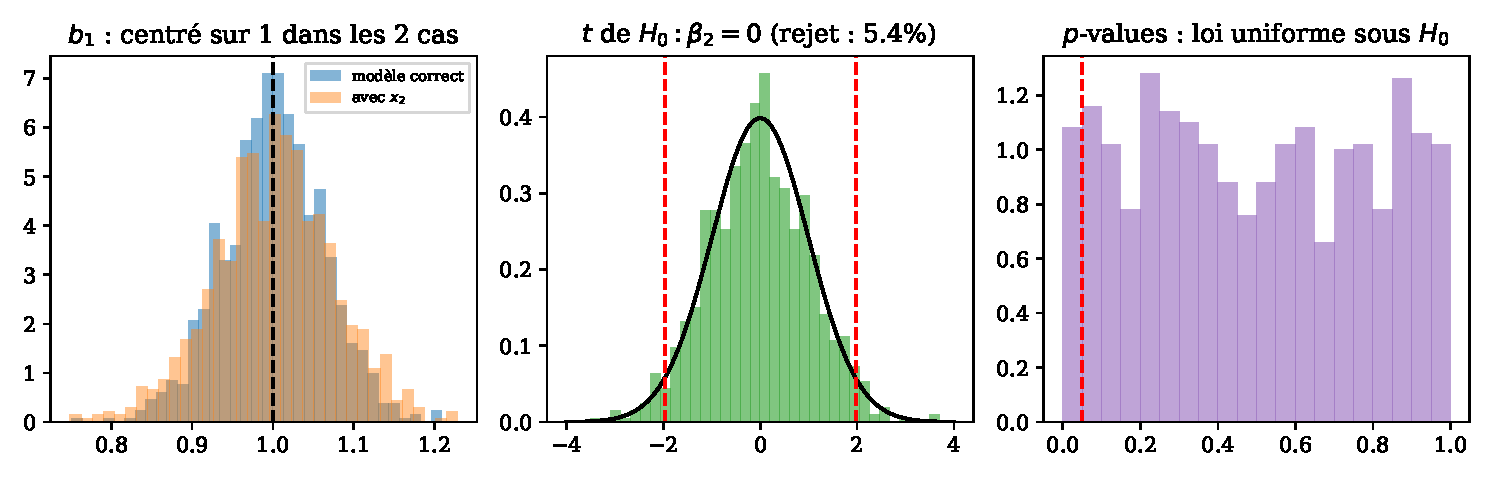
\includegraphics[width=\textwidth]{figures/q3_montecarlo.pdf}
\caption{Gauche : $b_1$ reste centré sur 1 mais est plus dispersé avec $x_2$. Centre : les 1000 statistiques $t$ de $H_0:\beta_2=0$ suivent la loi de Student à 247 degrés de liberté ; les zones de rejet sont au-delà des lignes rouges. Droite : les $p$-values sont uniformes sur $[0,1]$, donc environ 5\,\% tombent sous 0,05.}
\end{figure}

\textbf{Résultat.} On rejette $H_0$ dans \textbf{54 répétitions sur 1000, soit 5,4\,\%}.

\begin{reponse}
Non, on n'« accepte » pas $H_0$ à chaque répétition, bien que $H_0$ soit \emph{vraie} par construction. On la rejette dans 5,4\,\% des cas, soit environ $\alpha=5\,\%$.

\textbf{Explication.} Le niveau de signification $\alpha$ est, par définition, la probabilité de rejeter $H_0$ lorsqu'elle est vraie : c'est la probabilité d'une \textbf{erreur de type I}. Sous $H_0$ (et avec des erreurs normales), $t=b_2/\text{e.t.}(b_2)$ suit exactement une loi de Student à $n-3$ degrés de liberté. Il tombe donc dans la zone de rejet $|t|>1{,}970$ avec une probabilité d'exactement 5\,\%. Sur 1000 répétitions, on s'attend à environ 50 rejets « à tort ».

\textbf{Le 5,4\,\% est-il compatible avec 5\,\% ?} Le nombre de rejets suit une loi binomiale $(1000;\,0{,}05)$, dont l'écart-type de la proportion vaut $\sqrt{0{,}05\times0{,}95/1000}=0{,}0069$. L'intervalle $0{,}05\pm1{,}96\times0{,}0069=[3{,}6\,\%;\ 6{,}4\,\%]$ contient 5,4\,\%. Le test a donc bien la « taille » annoncée.

\textbf{Terminologie.} On dit « on ne rejette pas $H_0$ » plutôt que « on accepte $H_0$ » : ne pas rejeter ne prouve pas que $H_0$ est vraie.
\end{reponse}

% =====================================================================
\section{Question 4 (30 points) -- Rendement de l'éducation}
% =====================================================================

\begin{attention}[title={Note sur les données}]
Le fichier \texttt{assign2School.raw} n'était pas joint ; seul le dictionnaire l'était. Ses 34 variables (\texttt{id nearc2 nearc4 educ age \dots\ lwage expersq}) sont, dans le même ordre, celles du fichier \textbf{CARD} de Wooldridge (données de D. Card, 1995, sur 3010 hommes de la \emph{National Longitudinal Survey of Young Men}, salaires de 1976). Les résultats ci-dessous ont été calculés sur ce fichier ($n=3010$). \textbf{Relancez le do-file sur votre fichier} : si c'est bien le même, vous obtiendrez exactement ces chiffres.

Lecture des données dans Stata :\ \texttt{infile using dictionary.raw, using(assign2School.raw) clear}
\end{attention}

\subsection{(a) Régression de base et interprétation}

\begin{center}
\begin{tabular}{@{}lrrrr@{}}
\toprule
\texttt{lwage} & Coefficient & É.-t. & $t$ & $p$ \\
\midrule
\texttt{educ} & 0,09317 & 0,00361 & 25,80 & 0,000 \\
\texttt{exper} & 0,04066 & 0,00233 & 17,42 & 0,000 \\
constante & 4,66604 & 0,06379 & 73,15 & 0,000 \\
\midrule
\multicolumn{5}{@{}l}{$n=3010$, \ $R^2=0{,}181$, \ SCE $=485{,}18$, \ $s=0{,}4017$} \\
\bottomrule
\end{tabular}
\end{center}

\textbf{Comment interpréter un coefficient quand $y$ est en logarithme.} Dans $\ln w=\beta_0+\beta_1\,educ+\beta_2\,exper+\epsilon$, on a $\partial\ln w/\partial educ=\beta_1$. Une variation de $\Delta$ du log correspond à une variation relative d'environ $100\Delta\,\%$ (car $\ln(1+g)\approx g$ pour $g$ petit). La variation exacte est $100(e^{\Delta}-1)\,\%$.

\begin{reponse}
\begin{itemize}
\item \textbf{Éducation} : \emph{à expérience égale}, une année de scolarité supplémentaire est associée à un salaire plus élevé d'environ \textbf{9,3\,\%} (exactement $e^{0{,}0932}-1=9{,}8\,\%$). C'est le « rendement de l'éducation » au sens de Mincer.
\item \textbf{Expérience} : \emph{à éducation égale}, une année d'expérience supplémentaire est associée à un salaire plus élevé d'environ \textbf{4,1\,\%} (exactement 4,15\,\%).
\item « À \dots\ égale » est essentiel : par FWL, $b_{educ}$ ne mesure que la relation entre le salaire et la partie de l'éducation non expliquée par l'expérience.
\item Les deux coefficients sont très significatifs ($t=25{,}8$ et $17{,}4$).
\item \textbf{Prudence causale} : il s'agit d'une association. Si l'habileté (dans $\epsilon$) est corrélée à l'éducation, $\E[\epsilon\mid educ]\ne0$ et $b_{educ}$ est biaisé, probablement vers le haut (question 1(c)). C'est pour traiter ce problème que Card utilise la proximité d'un collège (\texttt{nearc4}) comme instrument.
\item L'unité du salaire (dollars ou cents) n'affecte que la constante, car $\ln(100w)=\ln100+\ln w$ ; voir la question 1(a).
\end{itemize}
\end{reponse}

\subsection{(b) Moyenne des résidus}

Résultat : $\bar e=-1{,}5\times10^{-15}$, c'est-à-dire \textbf{zéro} à la précision de l'ordinateur près.

\begin{reponse}
La moyenne des résidus est nulle, mais \textbf{ce n'est pas informatif} sur la moyenne des erreurs dans la population.
\begin{itemize}[nosep]
\item C'est une \textbf{propriété numérique} des MCO. La régression contient une constante, et la première équation normale ($\bm\iota'\ve=0$) impose $\sum e_i=0$ \emph{par construction}, quelles que soient les données et que le modèle soit bon ou mauvais (propriété 2 des notes, [26]).
\item Les résidus sont des \emph{estimations} des erreurs, calculées \emph{de façon à} sommer à zéro. Ils ne peuvent donc pas nous renseigner sur $\E[\epsilon]$ ni sur $\E[\epsilon\mid educ,exper]$.
\item De plus, comme montré en 1(c), une moyenne non nulle des erreurs ($\alpha_0$) serait absorbée par la constante : $\E[\epsilon]=0$ est une \emph{normalisation}, non testable. Ce qui compte pour l'absence de biais, c'est $\E[\epsilon\mid\vX]$ ne dépendant pas de $\vX$, et cela ne se vérifie pas avec les résidus (ils sont aussi orthogonaux à $educ$ et $exper$ par construction : $\vX'\ve=\mathbf 0$).
\end{itemize}
\end{reponse}

\subsection{(c) Test $H_0:\beta_{educ}=0{,}07$ par un test $t$}

\textbf{Démarche.}
\begin{enumerate}[nosep]
\item Hypothèses : $H_0:\beta_{educ}=0{,}07$ contre $H_a:\beta_{educ}\ne0{,}07$ (test bilatéral), au seuil $\alpha=5\,\%$.
\item Statistique : $t=\dfrac{b_{educ}-0{,}07}{\text{e.t.}(b_{educ})}$, qui suit sous $H_0$ une loi de Student à $n-k=3010-3=3007$ degrés de liberté.
\item Calcul : $t=\dfrac{0{,}093168-0{,}07}{0{,}003612}=\dfrac{0{,}023168}{0{,}003612}=\mathbf{6{,}41}$.
\item Valeur critique : $t_{0{,}975;\,3007}=1{,}961$. Comme $|6{,}41|>1{,}961$, on rejette $H_0$.
\item $p$-value : $p=2\,P(T_{3007}>6{,}41)=\mathbf{1{,}6\times10^{-10}}$.
\end{enumerate}
En Stata : \texttt{display 2*ttail(e(df\_r), abs((\_b[educ]-0.07)/\_se[educ]))}. Vérification possible avec \texttt{test educ = 0.07} (qui affiche $F=t^2=41{,}15$ et la même $p$-value) ou avec \texttt{lincom educ - 0.07}.

\begin{reponse}
$t=6{,}41$ et $p\approx1{,}6\times10^{-10}$ : on \textbf{rejette} $H_0$ à tous les niveaux usuels (1\,\%, 5\,\%, 10\,\%). Le rendement estimé (9,3\,\%) est significativement supérieur aux 7\,\% du collègue.

\textbf{Interprétation de la $p$-value} : si le vrai rendement était de 0,07, la probabilité d'obtenir, dans un échantillon comme le nôtre, une estimation au moins aussi éloignée de 0,07 que celle observée ($|t|\ge6{,}41$) serait d'environ 1,6 sur 10 milliards. Une telle observation est pratiquement incompatible avec $H_0$. C'est aussi le plus petit seuil $\alpha$ auquel on rejetterait $H_0$.

\textbf{Cohérence} : l'intervalle de confiance à 95\,\%, $[0{,}086;\ 0{,}100]$, ne contient pas 0,07.

\textbf{Nuance} : la $p$-value n'est \emph{pas} la probabilité que $H_0$ soit vraie.
\end{reponse}

\subsection{(d) Reparamétrisation}

\begin{idee}
Le tableau de régression donne automatiquement le test de « coefficient $=0$ ». On réécrit donc le modèle pour qu'un coefficient soit égal à $\theta=\beta_{educ}-0{,}07$ : tester $\theta=0$ revient alors à tester $\beta_{educ}=0{,}07$.
\end{idee}

On pose $\theta=\beta_1-0{,}07$, soit $\beta_1=\theta+0{,}07$. On remplace dans le modèle :
\[
lwage=\beta_0+(\theta+0{,}07)\,educ+\beta_2\,exper+\epsilon
\iff
\underbrace{lwage-0{,}07\,educ}_{\text{nouvelle variable dépendante}}=\beta_0+\theta\,educ+\beta_2\,exper+\epsilon .
\]
\begin{lstlisting}
generate lwage_r = lwage - 0.07*educ
regress lwage_r educ exper
\end{lstlisting}
\begin{center}
\begin{tabular}{@{}lrrrr@{}}
\toprule
\texttt{lwage\_r} & Coefficient & É.-t. & $t$ & $p$ \\
\midrule
\texttt{educ} ($=\hat\theta$) & 0,02317 & 0,00361 & \textbf{6,41} & \textbf{0,000} \\
\texttt{exper} & 0,04066 & 0,00233 & 17,42 & 0,000 \\
constante & 4,66604 & 0,06379 & 73,15 & 0,000 \\
\bottomrule
\end{tabular}
\end{center}

\begin{reponse}
Le coefficient de \texttt{educ} vaut maintenant $\hat\theta=0{,}0932-0{,}07=0{,}0232$, avec le \emph{même} écart-type (0,00361). La ligne \texttt{educ} du tableau affiche directement $t=6{,}41$ et $p=0{,}000$ ($1{,}6\times10^{-10}$), les mêmes valeurs qu'en (c). Les autres coefficients sont inchangés.

Pourquoi l'écart-type ne change pas : soustraire $0{,}07\,educ$ à $y$ ne modifie ni $\vX$ ni les résidus ($y-0{,}07\,educ-\hat\beta_0-\hat\theta\,educ-\hat\beta_2\,exper=e$), donc ni $s^2$ ni $s^2(\vX'\vX)^{-1}$.
\end{reponse}

\subsection{(e) Différence de salaire constante entre le Sud et ailleurs}

\begin{idee}
« Différence constante et indépendante de l'éducation et de l'expérience » : on ajoute une variable indicatrice \texttt{south}, qui ne déplace que la constante (deux droites parallèles). On teste ensuite la nullité de son coefficient.
\end{idee}

Modèle : $lwage=\beta_0+\beta_1\,educ+\beta_2\,exper+\delta\,south+\epsilon$.
Hors du Sud, la constante est $\beta_0$ ; dans le Sud, elle est $\beta_0+\delta$. Les pentes sont les mêmes.
$H_0:\delta=0$ (salaires identiques à éducation et expérience égales) contre $H_a:\delta\ne0$.

\begin{center}
\begin{tabular}{@{}lrrrr@{}}
\toprule
\texttt{lwage} & Coefficient & É.-t. & $t$ & $p$ \\
\midrule
\texttt{educ} & 0,08492 & 0,00356 & 23,86 & 0,000 \\
\texttt{exper} & 0,03983 & 0,00227 & 17,57 & 0,000 \\
\texttt{south} & $-0{,}20074$ & 0,01480 & $-13{,}57$ & 0,000 \\
constante & 4,86370 & 0,06362 & 76,45 & 0,000 \\
\midrule
\multicolumn{5}{@{}l}{$n=3010$, \ $R^2=0{,}229$, \ SCE $=457{,}19$} \\
\bottomrule
\end{tabular}
\end{center}

\begin{reponse}
$t=-0{,}2007/0{,}0148=-13{,}57$, $p<0{,}0001$ (valeur critique 1,961) : on \textbf{rejette} $H_0$. À éducation et expérience égales, les salaires dans le Sud sont inférieurs d'environ \textbf{20\,\%} (exactement $e^{-0{,}2007}-1=-18{,}2\,\%$) à ceux des autres régions.

On peut aussi faire le test par un $F$ (\texttt{test south}) : $F=t^2=184{,}1$, même conclusion. Le résultat est robuste à l'hétéroscédasticité (\texttt{vce(robust)} : $t=-13{,}4$).

Remarque : l'ajout de \texttt{south} fait baisser le rendement estimé de l'éducation (de 0,093 à 0,085). Le Sud a en moyenne moins d'éducation \emph{et} des salaires plus bas ; en (a), une partie de l'effet régional était attribuée à l'éducation (biais de variable omise).
\end{reponse}

\subsection{(f) Marchés du travail identiques ? Test de Chow}

\begin{idee}
On permet à \emph{tous} les coefficients (constante, rendement de l'éducation, rendement de l'expérience) de différer entre le Sud et ailleurs, en interagissant chaque variable avec \texttt{south}. « Marchés identiques » signifie que les trois différences sont nulles : c'est une hypothèse jointe (3 restrictions), qu'on teste avec un $F$. C'est le \textbf{test de Chow}.
\end{idee}

\textbf{Modèle non contraint.}
\[
lwage=\beta_0+\beta_1 educ+\beta_2 exper+\delta_0\,south+\delta_1\,(south\times educ)+\delta_2\,(south\times exper)+\epsilon .
\]
Hors du Sud : constante $\beta_0$, pentes $\beta_1,\beta_2$. Dans le Sud : $\beta_0+\delta_0$, $\beta_1+\delta_1$, $\beta_2+\delta_2$.
\[
H_0:\ \delta_0=\delta_1=\delta_2=0\qquad\text{contre}\qquad H_a:\ \text{au moins un }\delta_j\ne0 .
\]

\begin{center}
\begin{tabular}{@{}lrrrr@{}}
\toprule
\texttt{lwage} & Coefficient & É.-t. & $t$ & $p$ \\
\midrule
\texttt{educ} & 0,07312 & 0,00462 & 15,84 & 0,000 \\
\texttt{exper} & 0,04471 & 0,00289 & 15,49 & 0,000 \\
\texttt{south} & $-0{,}42419$ & 0,12677 & $-3{,}35$ & 0,001 \\
\texttt{south}$\times$\texttt{educ} & 0,02404 & 0,00722 & 3,33 & 0,001 \\
\texttt{south}$\times$\texttt{exper} & $-0{,}01032$ & 0,00462 & $-2{,}23$ & 0,026 \\
constante & 4,98414 & 0,08079 & 61,69 & 0,000 \\
\midrule
\multicolumn{5}{@{}l}{$n=3010$, \ $R^2=0{,}240$, \ SCE$_{NC}=450{,}24$, \ $n-k=3004$} \\
\bottomrule
\end{tabular}
\end{center}

\textbf{Statistique $F$ à la main.} Le modèle contraint (sous $H_0$) est celui de (a) : SCE$_C=485{,}18$. Avec $q=3$ restrictions et $n-k=3010-6=3004$ :
\[
F=\frac{(\text{SCE}_C-\text{SCE}_{NC})/q}{\text{SCE}_{NC}/(n-k)}=\frac{(485{,}18-450{,}24)/3}{450{,}24/3004}=\frac{11{,}647}{0{,}14988}=\mathbf{77{,}7}.
\]
Valeur critique $F_{0{,}95;\,3;\,3004}=2{,}61$ ; $p$-value $\approx2\times10^{-48}$.

\textbf{Vérification par régressions séparées.} La régression interagie équivaut à estimer le modèle séparément dans chaque région :
\begin{itemize}[nosep]
\item Sud ($n=1215$) : $\widehat{lwage}=4{,}560+0{,}0972\,educ+0{,}0344\,exper$, SCE $=185{,}90$ ;
\item ailleurs ($n=1795$) : $\widehat{lwage}=4{,}984+0{,}0731\,educ+0{,}0447\,exper$, SCE $=264{,}34$.
\end{itemize}
On vérifie $185{,}90+264{,}34=450{,}24=\text{SCE}_{NC}$. C'est la forme classique du test de Chow.

\begin{reponse}
$F=77{,}7>2{,}61$ ($p\approx0$) : on \textbf{rejette} fortement l'hypothèse que les marchés du travail du Sud et du reste du pays sont identiques. Les différences ne se limitent pas à la constante :
\begin{itemize}[nosep]
\item \textbf{rendement de l'éducation plus élevé dans le Sud} : 9,7\,\% contre 7,3\,\% par année d'étude (différence de 2,4 points, $t=3{,}33$, significative) ;
\item \textbf{rendement de l'expérience plus faible dans le Sud} : 3,4\,\% contre 4,5\,\% par année (différence de $-1{,}0$ point, $t=-2{,}23$, significative à 5\,\%) ;
\item \textbf{l'écart salarial dépend donc du profil} : il vaut $-0{,}424+0{,}024\,educ-0{,}010\,exper$. Pour $educ=12$ et $exper=8$ : $-0{,}218$ (environ $-20\,\%$). Pour $educ=16$ et $exper=8$ : $-0{,}122$ (environ $-11\,\%$). L'écart se réduit pour les plus éduqués.
\end{itemize}
Un test des seules pentes ($\delta_1=\delta_2=0$) rejette aussi l'égalité ($F=23{,}2$, $p\approx10^{-10}$). L'hypothèse de (e) d'une différence constante est donc elle-même rejetée : le modèle (e) est trop restrictif.

\textbf{Mise en garde} : le test de Chow classique suppose la même variance des erreurs dans les deux régions. Une version robuste à l'hétéroscédasticité (\texttt{vce(robust)} puis \texttt{test}) donne $F=77{,}3$ : la conclusion est inchangée.
\end{reponse}

% =====================================================================
\section*{Annexe -- Code Stata}
\addcontentsline{toc}{section}{Annexe -- Code Stata}
Le fichier complet et commenté est \texttt{stata/devoir1.do}. Structure :
\begin{lstlisting}
* Q3 : set seed 1234 ; x1, x2 fixes ; boucle de 1000 répétitions ;
*      post des b, se, et du rejet de H0: beta2=0 ; puis summarize / ttest
* Q4 : infile using dictionary.raw, using(assign2School.raw) clear
*   (a) regress lwage educ exper
*   (b) predict uhat, residuals ; summarize uhat
*   (c) display (_b[educ]-0.07)/_se[educ] ; 2*ttail(e(df_r),abs(t)) ; test educ=0.07
*   (d) generate lwage_r = lwage - 0.07*educ ; regress lwage_r educ exper
*   (e) regress lwage educ exper south
*   (f) regress lwage c.educ##i.south c.exper##i.south
*       test 1.south 1.south#c.educ 1.south#c.exper   (+ Chow à la main)
\end{lstlisting}

\end{document}
